%=======================+=========================
%==============  DAQ   ================
%=================================================\

\section[Data Acquisition]{Data acquisition \label{sec:daq}}

%\subsection{Architecture \label{sec:daqarchitecture}}

%\subsection{Performance \label{sec:daqperformance}}

The GlueX data acquisition uses the CEBAF Data Acquisition (CODA) framework. CODA is a software toolkit of applications and libraries that allows one to build customized data acquisition systems based on distributed commercial networks. A detailed description of CODA software and hardware can be found in Ref.\,\cite{CLAS12_DAQ}. 
The electronics in the VME/VXS crate can produce data up to 200 MB/s per crate and the
number of crates producing data is about 55.
The data from the electronic modules are read via the VME back-plane (2eSST, parallel bus) by the crate readout controller (ROC), which is a single board computer running Linux.
The \gx~ network layout and data flow are shown on Fig.~\ref{fig:CODA}.
Typical data rates from a %=======================+=========================

single crate are in the range of 10--70~MB/s, depending on the detector type and trigger rate.
The ROC transfers data over 1~Gbit Ethernet link to Data Concentrators (DC) 40 event fragments at a time. Data Concentrators are programs, which build partial events received from 10-12 crates and run on a dedicated computer node.
The DC output traffic of 200-600 MB/s is routed to the Event Builder (EB) to build complete events.
The Event Recorder (ER), which is typically running on the same node as an event builder, write data to the local data storage.
To date, GlueX data has collected at a rate of 500--900 MB/s, which allows the ER to write out to a single output stream. The system is expandable to handle higher luminosity with rates of 1.5--2.5~GB/s. In this case, the ER must write multi-stream data to several files in parallel.
All DAQ nodes {\color{red} Elton: nodes same as CPUs / ROCs? } are connected to both a 40 Gb Ethernet switch and a 56 Gb Infiniband switch.
The ethernet network is used exclusively for DAQ purposes: receiving data from detectors, building events, and writing data to disk, 
while the Infiniband network is used to transfer events for online data quality monitoring. 
This allows one to decouple DAQ and monitoring network traffic.
The live time of the DAQ is in the range of 92--100\%. The dead time is coming from readout electronics and depends on the trigger rate.  
The software part of DAQ has no dead time during the run, but it appears while stopping and starting the run, at the level of 2-8 minutes. 



\begin{figure}[tbp]
\begin{center}
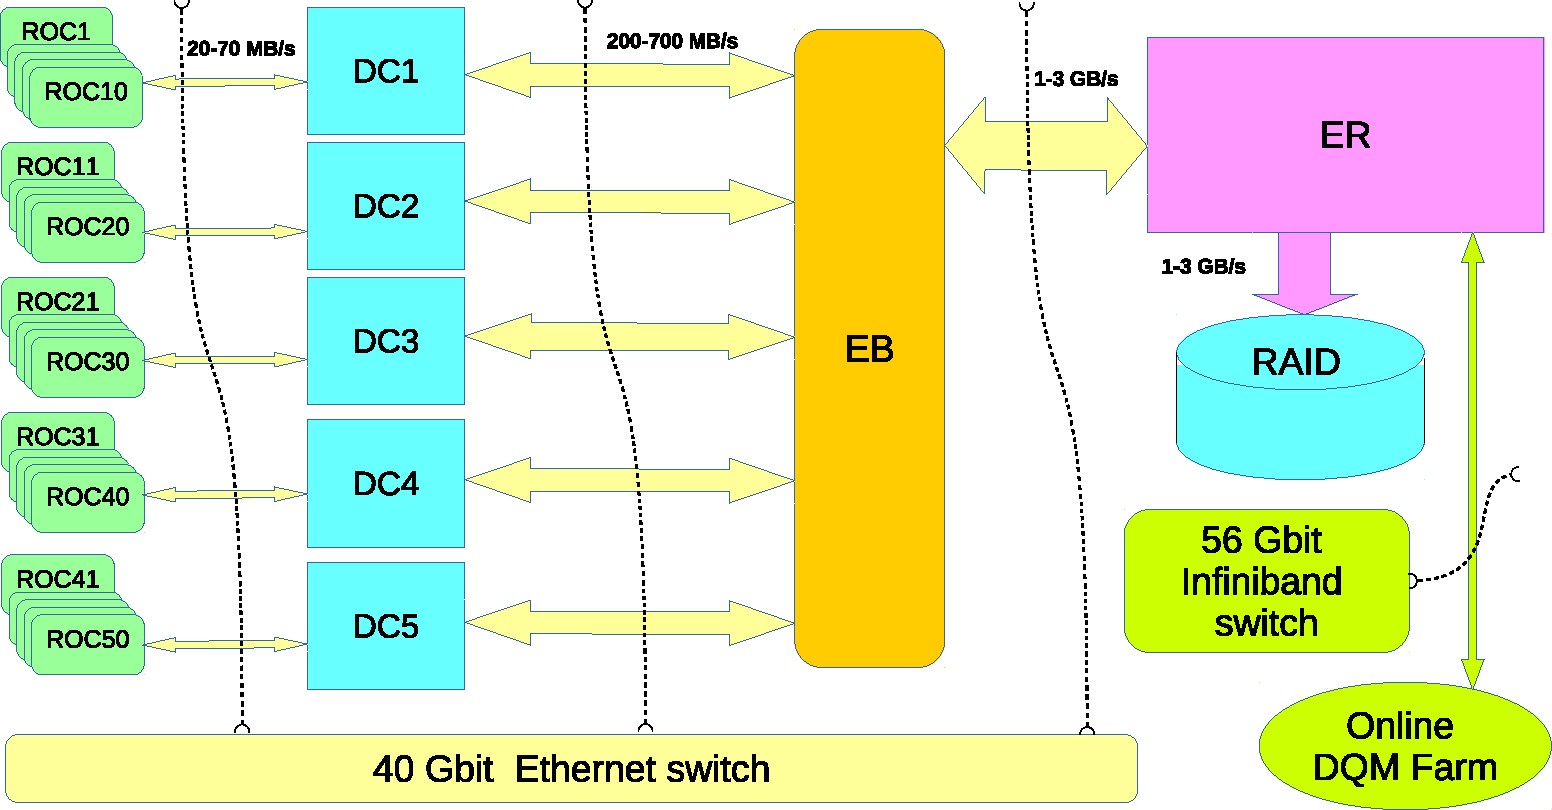
\includegraphics[width=0.75\textwidth]{figures/DAQ_coda.pdf}  
\caption{ \label{fig:CODA}
DAQ layout}

\end{center}
\end{figure}
